\chapter{RESULTS AND DISCUSSION}
The performance of the proposed AI-based multi-label food spoilage detection system is evaluated using deep learning performance metrics, visualization techniques, IoT sensor analysis, and Explainable AI outputs. The trained models are tested on unseen images to evaluate their ability to classify fruits and vegetables into Fresh, Early Spoilage, Moderate Spoilage, and Severe Spoilage stages. The evaluation process includes analysis of training and validation performance, confusion matrix interpretation, ROC analysis, Grad-CAM visualization, and IoT sensor monitoring results. This chapter discusses the experimental results obtained from the proposed system and analyzes the effectiveness of the implemented methodologies.

\section[Dataset Distribution and Visualization]{\textbf{Dataset Distribution and Visualization}}
The dataset used for training and evaluation consists of fruit and vegetable images categorized into four spoilage stages. The dataset is divided into training, validation, and testing sets using a standard split ratio to ensure effective model training and unbiased evaluation. Data augmentation techniques such as rotation, flipping, zooming, and brightness adjustment are applied to improve dataset diversity and model robustness.

Visualization of the dataset distribution helps analyze class balance and spoilage stage representation. Sample image grids are generated for all spoilage stages to verify dataset quality and labeling consistency. Pixel intensity distribution analysis is also performed to understand visual variations between spoilage stages.

\begin{table}[H]
	\centering
	\caption{Dataset Distribution}
	\label{tab:dataset_distribution}
	\begin{tabular}{|l|l|}
		\hline
		\textbf{Dataset} & \textbf{Split Percentage} \\ \hline
		Training Set & 70\% \\ \hline
		Validation Set & 15\% \\ \hline
		Testing Set & 15\% \\ \hline
	\end{tabular}
\end{table}

\section[Model Training and Validation Performance]{\textbf{Model Training and Validation Performance}}
The proposed food spoilage detection system was trained and evaluated using four deep learning architectures: CustomCNN, MobileNetV2, ResNet50, and EfficientNetB0. All models were trained using the same 70:15:15 dataset split, identical augmentation techniques, class weights, and preprocessing pipeline to ensure fair comparison. Performance evaluation was carried out using Accuracy, Precision, Recall, F1-Score, and ROC-AUC metrics.

The comparative analysis results indicate that MobileNetV2 achieved the best overall performance among all evaluated models. MobileNetV2 obtained an accuracy of 62.75\%, precision of 72.05\%, recall of 62.75\%, F1-score of 65.47\%, and ROC-AUC value of 85.74\%. The model demonstrated better generalization capability and more stable classification performance across different spoilage stages compared to the other architectures. The lightweight architecture and depthwise separable convolution operations used in MobileNetV2 improved feature extraction efficiency while maintaining lower computational complexity.

The CustomCNN model achieved moderate performance with an accuracy of 34.07\%, precision of 62.45\%, recall of 34.07\%, F1-score of 33.44\%, and ROC-AUC value of 80.71\%. Although the model showed lower classification accuracy compared to transfer learning architectures, it demonstrated good ROC performance and faster inference capability because of its smaller architecture size. The CustomCNN model served as a baseline architecture for comparison against pretrained transfer learning models.

ResNet50 achieved an accuracy of 51.47\%, precision of 39.88\%, recall of 51.47\%, F1-score of 37.46\%, and ROC-AUC value of 64.04\%. The model demonstrated strong feature extraction capability for Fresh samples but showed difficulty in correctly distinguishing Early Spoilage and Severe Spoilage stages. The deeper architecture increased model complexity and training time without providing significant improvement in classification performance for the current dataset.

EfficientNetB0 also achieved an accuracy of 51.47\% with a precision of 30.15\%, recall of 51.47\%, F1-score of 36.17\%, and ROC-AUC value of 51.47\%. Although EfficientNetB0 is known for parameter efficiency and optimized scaling, the model showed inconsistent classification performance for the present multi-label spoilage dataset. The results suggest that EfficientNetB0 may require larger datasets and further hyperparameter tuning for improved performance in spoilage classification tasks.

\begin{figure}[H]
	\centering
	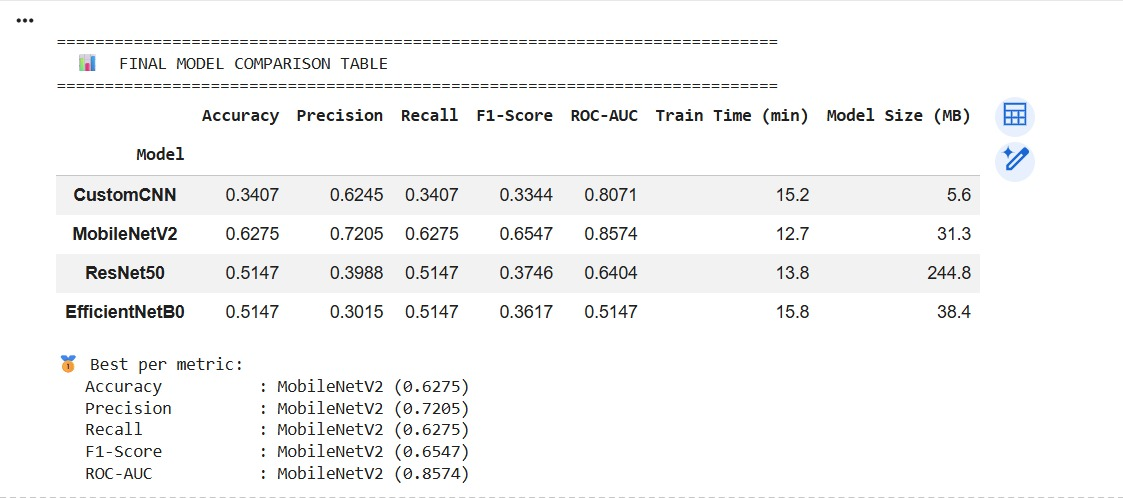
\includegraphics[width=1\textwidth]{Figures/performance_table}
	\caption{Final comparative performance analysis of deep learning models including training time and model size.}
	\label{fig:performance_table_img}
\end{figure}

\begin{figure}[H]
	\centering
	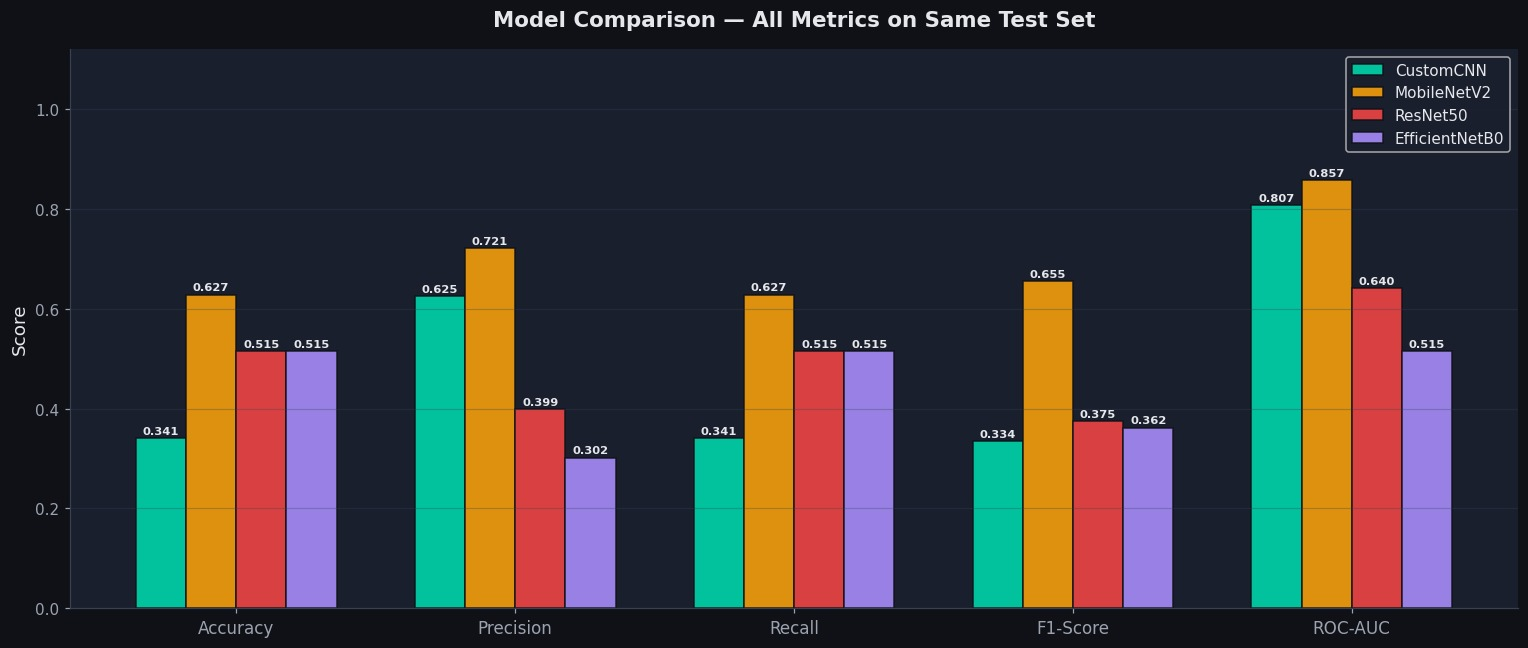
\includegraphics[width=1\textwidth]{Figures/performance_bar_chart}
	\caption{Model comparison across all metrics on the same test set.}
	\label{fig:performance_bar_chart_img}
\end{figure}

\begin{table}[H]
	\centering
	\caption{Comparative Performance Analysis of Deep Learning Models}
	\label{tab:model_comparison}
	\begin{tabular}{|l|c|c|c|c|c|}
		\hline
		\textbf{Model} & \textbf{Accuracy} & \textbf{Precision} & \textbf{Recall} & \textbf{F1-Score} & \textbf{ROC-AUC} \\ \hline
		CustomCNN & 34.07\% & 62.45\% & 34.07\% & 33.44\% & 80.71\% \\ \hline
		MobileNetV2 & 62.75\% & 72.05\% & 62.75\% & 65.47\% & 85.74\% \\ \hline
		ResNet50 & 51.47\% & 39.88\% & 51.47\% & 37.46\% & 64.04\% \\ \hline
		EfficientNetB0 & 51.47\% & 30.15\% & 51.47\% & 36.17\% & 51.47\% \\ \hline
	\end{tabular}
\end{table}

\section[Confusion Matrix and Classification Analysis]{\textbf{Confusion Matrix and Classification Analysis}}
Confusion matrix analysis was performed to evaluate stage-wise classification capability of the trained models. The confusion matrices indicate that MobileNetV2 provided the most balanced classification performance across all spoilage stages. The model correctly identified Fresh samples with high accuracy while also demonstrating improved prediction capability for Moderate and Severe Spoilage classes. Compared to the other architectures, MobileNetV2 produced fewer false classifications and achieved better class-wise balance.

The CustomCNN model showed moderate performance for Severe Spoilage classification but struggled to differentiate Early Spoilage and Moderate Spoilage stages accurately. ResNet50 and EfficientNetB0 strongly favored Fresh class predictions and misclassified many spoiled samples as Fresh, resulting in reduced F1-score and poor class-wise balance. This indicates that deeper architectures may require larger and more balanced datasets to effectively learn subtle spoilage variations between intermediate spoilage stages.

Per-class F1-score analysis further confirmed that MobileNetV2 achieved the best overall class-wise balance among all evaluated models. The model achieved higher F1-scores for Fresh, Moderate Spoilage, and Severe Spoilage classes compared to the remaining architectures. The results demonstrate that MobileNetV2 is the most suitable architecture for the current food spoilage detection dataset and implementation workflow.

\begin{figure}[H]
	\centering
	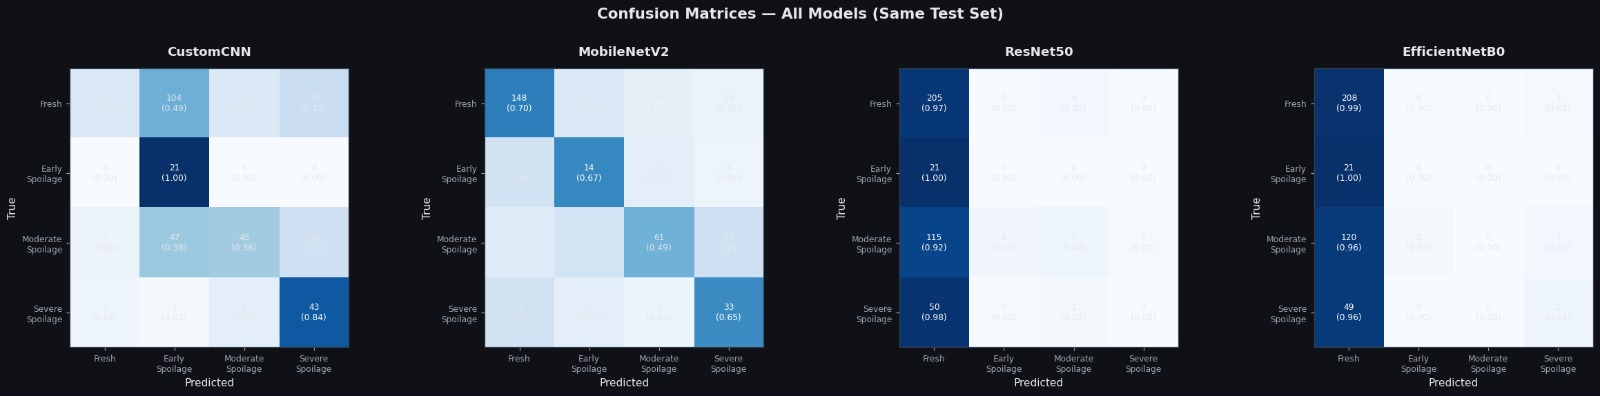
\includegraphics[width=1\textwidth]{Figures/confusion_matrices}
	\caption{Confusion Matrices for CustomCNN, MobileNetV2, ResNet50, and EfficientNetB0 on the same test set.}
	\label{fig:confusion_matrices_img}
\end{figure}

\begin{figure}[H]
	\centering
	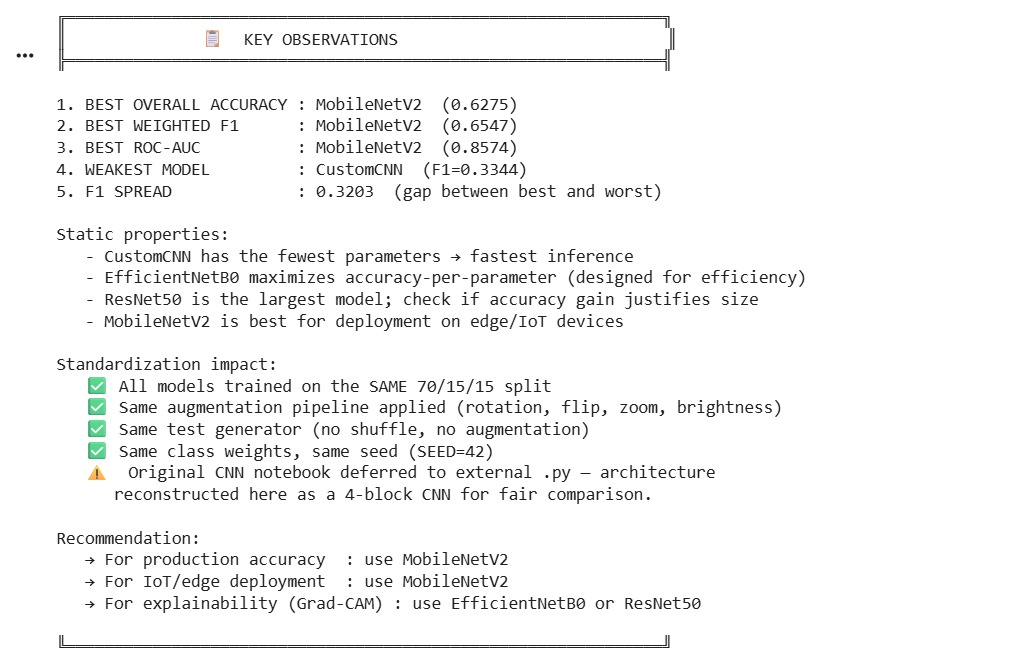
\includegraphics[width=0.8\textwidth]{Figures/key_observations}
	\caption{Key observations and summary of findings from the model evaluation.}
	\label{fig:key_observations_img}
\end{figure}

\begin{table}[H]
	\centering
	\caption{Key Observations from Comparative Analysis}
	\label{tab:key_observations}
	\begin{tabular}{|l|l|}
		\hline
		\textbf{Observation} & \textbf{Result} \\ \hline
		Best Overall Accuracy & MobileNetV2 (62.75\%) \\ \hline
		Best Weighted F1-Score & MobileNetV2 (65.47\%) \\ \hline
		Best ROC-AUC & MobileNetV2 (85.74\%) \\ \hline
		Fastest Lightweight Model & MobileNetV2 \\ \hline
		Weakest Overall Model & CustomCNN \\ \hline
		Largest Model Size & ResNet50 \\ \hline
	\end{tabular}
\end{table}

\section[ROC Curve and Per-Class Performance Analysis]{\textbf{ROC Curve and Per-Class Performance Analysis}}
ROC curve analysis was performed using a one-vs-rest classification strategy for all spoilage stages. The ROC curves indicate that MobileNetV2 achieved the highest Area Under Curve (AUC) values across most spoilage classes, demonstrating stronger class separability and prediction reliability. The model achieved particularly high ROC performance for Fresh and Severe Spoilage stages.

The CustomCNN model demonstrated acceptable ROC performance despite lower overall classification accuracy, indicating that the model was capable of learning important visual features but lacked strong class-wise generalization. ResNet50 and EfficientNetB0 produced weaker ROC curves for Early and Moderate Spoilage stages, suggesting difficulty in learning subtle spoilage transitions from the available dataset.

Per-class F1-score analysis revealed that Fresh samples were generally classified more accurately across all architectures because of their strong visual distinction. However, intermediate spoilage stages such as Early Spoilage and Moderate Spoilage were more difficult to classify due to overlapping visual characteristics and gradual spoilage progression. This highlights the complexity of multi-label food spoilage classification compared to conventional binary classification systems.

\begin{figure}[H]
	\centering
	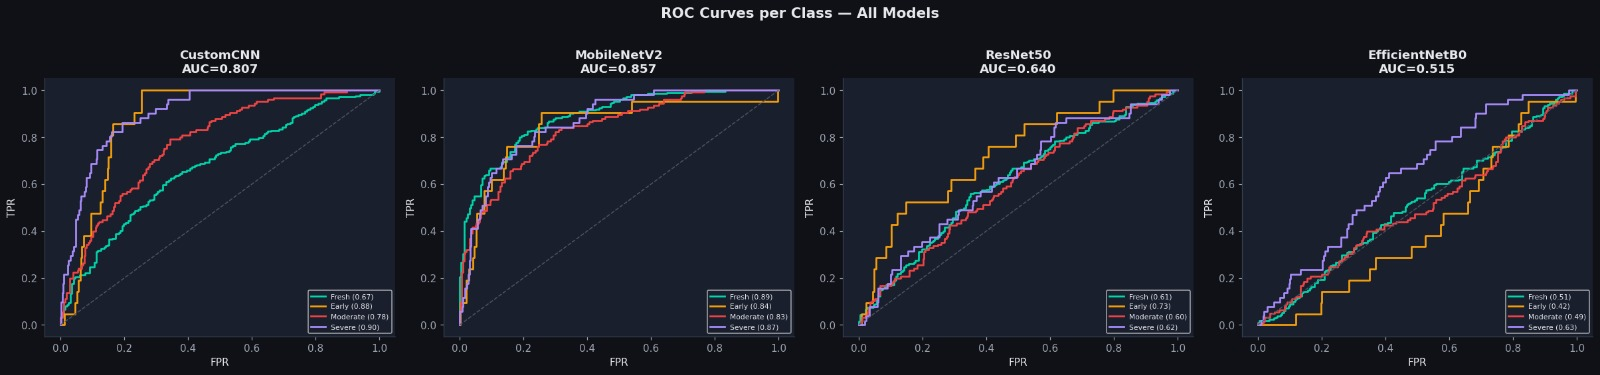
\includegraphics[width=1\textwidth]{Figures/roc_curves}
	\caption{ROC Curves per class for all evaluated deep learning models.}
	\label{fig:roc_curves_img}
\end{figure}
